\documentclass[russian,12pt,floatsection,nocolumnsxix]{eskdtext}


% закомментировать для рамок 
\usepackage[numbertop, numbercenter]{eskdplain}

\usepackage[utf8x]{inputenc}

\usepackage{setspace}
\onehalfspacing % полуторный интервал для всего текста

% - Подключаем шрифты из пакета scalable-cyrfonts-tex
\usepackage{cyrtimes}

% - Отступ красной строки
\setlength{\parindent}{1.25cm}

% - Убирает точку в списке литературы
\makeatletter
\def\@biblabel#1{#1 }

% ограничение для оглавления
%\usepackage{tocvsec2}
\setcounter{tocdepth}{2}

% - Точки для всех пунктов в оглавлении
\renewcommand*{\l@section}{\@dottedtocline{1}{1.5em}{2.3em}}
\renewcommand*{\l@subsection}{\@dottedtocline{1}{1.5em}{2.3em}}
\renewcommand*{\l@subsubsection}{\@dottedtocline{1}{1.5em}{2.3em}}

% - Для переопределения списков
\renewcommand{\theenumi}{\arabic{enumi}}
\renewcommand{\labelenumi}{\theenumi)}
\makeatother

\usepackage{enumitem}
\setlist{nolistsep, itemsep=0.3cm,parsep=0pt}

% - ГОСТ списка литературы
\bibliographystyle{utf8gost705u}


% - Верикальные отступы заголовков 
\ESKDsectSkip{section}{1em}{1em}
\ESKDsectSkip{subsection}{1em}{1em}
\ESKDsectSkip{subsubsection}{1em}{1em}

% - Изменение заголовков
\usepackage{titlesec}
\titleformat{\section}{\normalfont\normalsize\centering}{\thesection}{1.0em}{}
\titleformat{\subsection}{\normalfont\normalsize\centering}{\thesubsection}{1.0em}{}
\titleformat{\subsubsection}{\normalfont\normalsize\centering}{\thesubsubsection}{1.0em}{}
\titleformat{\paragraph}{\normalfont\normalsize\centering}{\theparagraph}{1.0em}{}

% - Оставим место под ТЗ 
\setcounter{page}{1}

% - Для больших таблиц
\usepackage{longtable}
\usepackage{tabularx}
\renewcommand{\thetable}{\thesection.\arabic{table}}

% - Используем графику в документе
\usepackage{graphicx}
\graphicspath{{images/}}
\renewcommand{\thefigure}{\thesection.\arabic{figure}}

% - Счётчики
\usepackage{eskdtotal}

% - Выравнивание по ширине
\sloppy

% - Разрешить перенос двух последних букв слова
\righthyphenmin=2

% - Оформление списков
\RequirePackage{enumitem}
\renewcommand{\alph}[1]{\asbuk{#1}}
\setlist{nolistsep}
\setitemize[1]{label=--, fullwidth, itemindent=\parindent, 
  listparindent=\parindent}% для дефисного списка
\setitemize[2]{label=--, fullwidth, itemindent=\parindent, 
  listparindent=\parindent, leftmargin=\parindent}
\setenumerate[1]{label=\arabic*), fullwidth, itemindent=\parindent, 
  listparindent=\parindent}% для нумерованного списка
\setenumerate[2]{label=\alph*), fullwidth, itemindent=\parindent, 
  listparindent=\parindent, leftmargin=\parindent}% для списка 2-ой ступени, который будет нумероваться а), б) и т.д.
  
% - Оформляем листинг кода (не использовать комментарии на русском!)
\usepackage{listings}  
\lstset{basicstyle=\ttfamily\scriptsize}
\lstset{extendedchars=\true}

% - выводим текст как есть с размером шрифта scriptsize
\makeatletter
\def\verbatim{\scriptsize\@verbatim \frenchspacing\@vobeyspaces \@xverbatim}
\makeatother

% - Вставка pdf
\usepackage[enable-survey]{pdfpages}

%межстрочный интервал
\usepackage{setspace}
\linespread{1.5}

%фамилии для рамок
\author{\ESKDfontII Мейта М.В.}
\ESKDchecker{\ESKDfontII Романов А.С.}
\ESKDnormContr{\ESKDfontII Якимук А.Ю.}
\ESKDapprovedBy{\ESKDfontII Шелупанов А.А.}
\ESKDcolumnI{\ESKDfontIII Разработка и тестирование программного обеспечения для оценки деформации поверхности твёрдых тел по серии оптических изображений}
\ESKDcolumnIX{\ESKDfontIII ТУСУР, ФБ, каф.~КИБЭВС, гр.~722}
\ESKDsignature{ЭСАУ.ДР.503390.001.ПЗ}

\begin{document}
\newpage
\ESKDthisStyle{empty}
%  
\includepdf[pages={1}]{title}
 \newpage
\ESKDthisStyle{empty}

\begin{center}
 \textbf{МИНИСТЕРСТВО ОБРАЗОВАНИЯ И НАУКИ РОССИЙСКОЙ ФЕДЕРАЦИИ}\\
 Федеральное государственное бюджетное образовательное учреждение высшего образования\\
 <<ТОМСКИЙ ГОСУДАРСТВЕННЫЙ УНИВЕРСИТЕТ СИСТЕМ УПРАВЛЕНИЯ И РАДИОЭЛЕКТРОНИКИ>> (ТУСУР)\\
 Кафедра комплексной информационной безопасности электронно-вычислительных систем (КИБЭВС)\\
\end{center} 

\vfill

\begin{flushright}
\begin{minipage}{0.45\textwidth}
 \begin{flushleft}
  К ЗАЩИТЕ ДОПУСТИТЬ\\
  заведующий каф. КИБЭВС\\
  д-р техн. наук, проф.\\
  \underline{\hspace{3cm}}А.А. Шелупанов \\
  <<\underline{\hspace{1cm}}>>\underline{\hspace{3cm}}2017г.\\
 \end{flushleft}
\end{minipage}
\end{flushright}

\vfill



\begin{center}
<<ОПРЕДЕЛЕНИЕ АВТОРСТВА ИСХОДНОГО КОДА>>

Специалистская работа по направлению 10.05.03 --

Информационная безопасность автоматизированных систем
\end{center}


\vfill


СОГЛАСОВАНО
\vspace{0.01cm}
\begin{singlespace}
 \begin{minipage}[left]{0.40\linewidth}
 Консультант по экономике:\\
 ст. преподаватель каф. КИБЭВС \\
 \underline{\hspace{2.5cm}}С.В. Глухарева \\
 "\underline{\hspace{1cm}}"\underline{\hspace{3cm}} 2017г.\\

 Консультант по безопасности\\ жизнедеятельности:\\
 канд. техн. наук, доцент каф. КИБЭВС\\
 \underline{\hspace{2.5cm}}Е.М. Давыдова\\
 "\underline{\hspace{1cm}}"\underline{\hspace{3cm}} 2017г.\\
 \end{minipage}
 \hfill
 \begin{minipage}[left]{0.5\linewidth}
  \vspace{0.7cm}
  Студент гр. 722 \\
  \underline{\hspace{3cm}}М.В. Мейта  \\
 "\underline{\hspace{1cm}}"\underline{\hspace{3cm}} 2017г.\\
 \vspace{0.3cm}\\ 
  Руководитель: \\
  канд. техн. наук, доцент каф. БИС \\
  \underline{\hspace{3cm}} А.С. Романов \\
  <<\underline{\hspace{1cm}}>>\underline{\hspace{3cm}}2017г.\\
 \end{minipage}
\end{singlespace}



% \begin{flushright}
% \begin{minipage}{0.45\textwidth}
%  \begin{flushleft}
%   Студент гр. 722 \\
%   \underline{\hspace{3cm}} Мейта М.В. \\
%   <<\underline{\hspace{1cm}}>>\underline{\hspace{3cm}}2017г.\\
%  \end{flushleft}
% \end{minipage}
% \end{flushright}
% 
% \vfill
% 
% \begin{flushright}
% \begin{minipage}{0.45\textwidth}
%  \begin{flushleft}
%   Руководитель: \\
%   канд. техн. наук, доцент каф. БИС \\
%   \underline{\hspace{3cm}} Романов А.С. \\
%   <<\underline{\hspace{1cm}}>>\underline{\hspace{3cm}}2017г.\\
%  \end{flushleft}
% \end{minipage}
% \end{flushright}

\vfill

\begin{center}
 ТОМСК 2017
\end{center}

 \ESKDthisStyle{empty}
 
\includepdf{practise_task}
 
\newpage
\ESKDthisStyle{empty}
\paragraph{\hfill РЕФЕРАТ \hfill}
Пояснительная записка содержит \ESKDtotal{page} страницы, \ESKDtotal{figure} рисунков, \ESKDtotal{table} таблиц, \ESKDtotal{bibitem} источников,
6 приложений.

% \ESKDtotal{table}
% \ESKDtotal{appendix}

СТИЛОМЕТРИЯ, ИСХОДНЫЙ КОД, ДЕАНОНИМИЗАЦИЯ АВТОРА, C/C++, КЛАССИФИКАЦИЯ, PYTHON, SKLEARN, JUPYTER NOTEBOOK, DECISION
TREES, RANDOM FOREST CLASSIFIER, КРОСС-ВАЛИДАЦИЯ, ADA BOOST, EXTREMLY RANDOMIZED TREES, GITHUB, LATEX.

Цель работы --- разработка программного обеспечения для определения авторства исходного кода программ
на языке C/C++, основанного на методах стилометрического анализа текста, с перспективой его
дальнейшего применения в борьбе с киберпреступностью, в области лицензионных, патентных и иных судебных разбирательств.

В рамках специалистской работы были поставлены следующие задачи: 
\begin{itemize}
  \item обзор существующих исследований, разработок, методов стилометрического анализа исходного кода программ;
\item построение модели процесса определения авторства исходного кода;
  \item разработка программного обеспечения для анализа исходного кода программ с применением стилометрии для
определения авторства программного обеспечения;
  \item подготовка и обработка тестового набора данных;
  \item исследование эффективности разработанной программы на основе модели анализа исходных кодов;
  \item анализ результатов;
  \item технико-экономическое обоснование работы;
  \item рассмотрение вопросов безопасности жизнедеятельности.
\end{itemize}

Объект исследования: деанонимизация автора программного обеспечения. 

Предмет исследования: стилометрия исходного кода программ на языках высокого уровня.

Достигнутые результаты: главным результатом специалистской работы является 
программное обеспечение <<WhoseCppCode>>, предназначенное для построения,
тестирования и оценки модели классификации авторов исходного кода на языке C/C++,
а также визуализации полученных результатов.

% \begin{itemize}
%   \item произведен аналитический обзор существующих методов анализа исходного кода программ с целью деанонимизации автора;
%   \item выбран набор признаков для классификации авторов программного кода на языке C/С++; 
%   \item выбраны алгоритмы классификации;
%   \item построена модель на определения авторства исходного кода;
%   \item разработано программное обеспечение для определения определения авторства  на языке программирования высокого уровня Python;
%   \item подготовлен тестовый набор данных;
%   \item реализован программный интерфейс с использованием технологии Jupyter Notebook;~\cite{jupyter}
%   \item выбраны критерии оценки эффективности разработанного алгоритма;
%   \item произведены вычислительные эксперименты на данном наборе данных;
%   \item сделаны выводы на основе полученных результатов.
% \end{itemize}

Пояснительная записка выполнена согласно ОС ТУСУР 01-2013~\cite{ostusur} при помощи системы компьютерной вёрстки \LaTeX. 

 \newpage
\ESKDthisStyle{empty}
\paragraph{\hfill ABSTRACT \hfill}
Explanatory note contains \ESKDtotal{page} pages, \ESKDtotal{figure} pictures, \ESKDtotal{table} tables,
\ESKDtotal{bibitem} sources, 7 appendicies.

STYLOMETRY, SOURCE CODE, AUTHORSHIP ATTRIBUTION, C/C++, CLASSIFICATION, PYTHON, SKLEARN,
JUPYTER NOTEBOOK, DECISION TREES, RANDOM FOREST CLASSIFIER, CROSS-VALIDATION, 
ADA BOOST, EXTREMLY RANDOMIZED TREES, GITHUB, LATEX.

The aim of this work is a software development of the tool for deanonimization of programmers, 
based on stylometry analysis of source code written in C/C++ programming language for future
usage in information security field: copyright/copyleft research, cybercrime investigation and patent licensing.

This specialist work solves the following tasks:
\begin{itemize}
  \item review of existing research, development, methods of stylometric analysis of source code;
  \item building a model for the process of determining the authorship of source code;
  \item software development of the system for source code analysis based on stylometry;
  \item development of software interface;
  \item preparation and processing of a test data set;
  \item study of the effectiveness of the developed program based on the analysis model of source codes;
  \item analysis of results;
  \item feasibility study;
  \item consideration of life safety issues.
\end{itemize}

Research object: deanonimization of the software developers.

Research subject: source code authorship attribution based on stylometry methods.

Achieved results: the main result of this work is developed software for C/C++ source code 
authorship attribution called <<WhoseCppCode>>.

Explanatory note is made using a word processor \LaTeX.

 
 % - содержание
 \newpage
 \ESKDstyle{plain}
 \tableofcontents

% \newpage
% \ESKDstyle{plain}
%  \addcontentsline{toc}{section}{Техническое задание}
% 
\section*{ТЕХНИЧЕСКОЕ ЗАДАНИЕ\\
на выполнение научно-исследовательских работ (НИР) по теме:\\
<<Определение авторства исходного кода>>}


\section{Основание для проведения НИР}

1.1\hspace{5mm}Положение о системе организации научно-исследовательской работы студентов ТУСУРа от 30.08.2013, положение о системе организации научно-исследовательской работы студентов ФБ.
 
1.2\hspace{5mm}Начало работ: 1 сентября 2016 г.

1.3\hspace{5mm}Срок окончания работ: 22 декабря 2016 г.

\section{Исполнители НИР}

Студент Томского государственного университета систем управления и радиоэлектроники (ТУСУР), кафедры комплексной информационной безопасности и электронно-вычислительных систем (КИБЭВС), 5 курса, гр. 722 Мейта Марина Валерьевна.

Научный руководитель: кандидат технических наук, доцент кафедры безопасности информационных систем (БИС) Романов Александр Сергеевич.

\section{Цель и задачи выполнения НИР}

Целью работы является разработка алгоритма для определения авторства программного обеспечения, основанного на стилометрическом анализе исходного кода программ на языках высокого уровня. Для достижения данной цели были поставлены следующие задачи:
\begin{itemize}
  \item обзор существующих исследований, разработок, методов стилометрического анализа текста, в том числе исходного кода программ; 
  \item разработка алгоритм анализа исходного кода программ с применением стилометрии для определения авторства программного обеспечения;
  \item создание программной реализации разработанного алгоритма;
  \item исследование эффективности разработанного алгоритма анализа исходных кодов.
\end{itemize}
Объект исследования: деанонимизация автора программного обеспечения.

Предмет исследования: стилометрия исходного кода программ на языках высокого уровня.   

\section{Научные и научно-технические результаты выполнения НИР}

4.1\hspace{5mm}При выполнении НИР должны быть получены следующие научно-технические результаты:

1)\hspace{5mm}результаты исследования методов определения авторства программного обеспечения, представленные в отчете о НИР, содержащим, в том числе:

а)\hspace{5mm}обзор и анализ современной научно-технической литературы, рассматривающей различные методы анализа текста и определения его авторства, основанные на стилометрии и применительные к деанонимизации автора исходного кода программ;

б)\hspace{5mm}формализованное описание разрабатываемого алгоритма для определения авторства исходного кода программ;

в)\hspace{5mm}код программы, реализующей алгоритм определения авторства исходного кода;

г)\hspace{5mm}исследование эффективности разработанного алгоритма;

д)\hspace{5mm}обобщение и выводы по результатам НИР;

е)\hspace{5mm}рекомендации и предложения по использованию результатов НИР.

2)\hspace{5mm}программная реализация разработанного алгоритма определения авторства исходного кода программ на языках высокого уровня с применением методов стилометрии.

\section{Основные требования к выполнению НИР}
\subsection{Требования к выполняемым работам}

5.1.1\hspace{5mm}В ходе выполнения НИР должны быть выполнены:

5.1.1\hspace{5mm}аналитический обзор существующих методов анализа текста, основанных на стилометрии;

5.1.2\hspace{5mm}разработка алгоритма определения авторства программного обеспечения с применением одного из изученных методов анализа текста;

5.1.3\hspace{5mm}программная реализация разработанного алгоритма;

5.1.4\hspace{5mm}исследование эффективности разработанного алгоритма;

5.1.5\hspace{5mm}написание научной статьи по проблеме, исследуемой в рамках НИР, объемом более 1 листа А4 или эквивалентном в листах другого размера.

\subsection{Требования к разрабатываемой документации}
5.2.1\hspace{5mm}В ходе работы должны быть разработаны и согласованы с научным руководителем и ответственным за НИР	 следующие документы:

5.2.1.1\hspace{5mm}заключительный отчет о НИР, оформленный в соответствии с ОС ТУСУР 01-2013;

5.2.1.2\hspace{5mm}проект технического задания на проведение НИР.

\section{Перечень и сроки выполнения этапов}
\subsection{Наименование этапов и выполняемые работы}
\subsection*{Этап 1. Обзор предметной области, постановка задачи}

1.1\hspace{5mm}Аналитический обзор информационных источников по теме стилометрического анализа текста.

1.2\hspace{5mm}Исследование методов стилометрического анализа текста применительно к исходному коду программ с целью деанонимизации автора исходного кода.

1.3\hspace{5mm}Подведение итогов этапа НИР.

\subsection*{Этап 2. Разработка алгоритма}
2.1\hspace{5mm}Разработка алгоритма определения авторства программного обеспечения на основе стилометрического анализа исходного кода программ;

2.2\hspace{5mm}Подведение итогов этапа НИР.

\subsection*{Этап 3. Программная реализация разработанного алгоритма}
3.1\hspace{5mm}Программная реализация разработанного алгоритма определения авторства программного обеспечения на основе стилометрического анализа исходного кода программ.

3.2\hspace{5mm}Исследование эффективности разработанного алгоритма, включающее в себя выбор критериев эффективности, формирование тестовых данных и проведение вычислительных экспериментов.

3.3\hspace{5mm}Подведение итогов этапа НИР.

\subsection*{Этап 4. Подведение итогов}
4.1\hspace{5mm}Обобщение и оценка полученных результатов, включающее в себя:
\begin{itemize}
  \item обобщение результатов исследований, в том числе исследования эффективности разработанного алгоритма определения авторства исходного кода программ;
  \item анализ выполнения требований технического задания на НИР;
  \item оценка полноты решения задач и достижения поставленных целей НИР.
\end{itemize}

4.2\hspace{5mm}Разработка отчета о НИР.

4.3\hspace{5mm}Подготовка результатов исследования к публикации.

\section{Предполагаемое использование результатов НИР}

7.1\hspace{5mm}Результаты проведенных НИР могут быть использованы специалистами по информационной безопасности, юристами и иными заинтересованными лицами для определения автора вредоносного программного обеспечения, подтверждения интеллектуальной собственности, отслеживания исходного кода после кибератаки, во время судебных разбирательств и т.п.

\section{Порядок выполнения и приемки этапов НИР}

8.1\hspace{5mm}Работы должны выполняться поэтапно в соответствии с настоящим техническим заданием.

8.2\hspace{5mm}Сдача и приемка выполненных работ (этапов работ) осуществляется в соответствии с календарным планом работ.

8.3\hspace{5mm}При приемке оценивается научно-технический уровень исследований, соответствие полученных результатов требованиям настоящего технического задания, обоснованность предлагаемых решений по реализации и использованию результатов НИР.

\begin{center}
  КАЛЕНДАРНЫЙ ПЛАН ВЫПОЛНЕНИЯ РАБОТ
\end{center}

\begin{table}[h]
\label{tab:3}
\begin{center}
\begin{tabular}{|c|c|c|}
\hline
Номер этапа & Начало периода & Окончание периода \\ 
\hline
Этап 1 & 01.09.2016 & 10.10.2016 \\
\hline
Этап 2 & 11.10.2016 & 07.11.2016 \\
\hline
Этап 3 & 08.11.2016 & 05.12.2016 \\
\hline
Этап 4 & 06.12.2016 & 22.12.2016 \\
\hline
\end{tabular}
\end{center}
\end{table}

\titleformat{\section}{\centering\normalfont\normalsize}{\thesection}{1.0em}{}

\newpage
\section*{
ЛИСТ СОГЛАСОВАНИЯ\\
к проекту технического задания\\
на выполнение научно-технической работы (НИР) по теме:\\
<<Определение авторства исходного кода>>}


\begin{flushleft}
\underline{\hspace{4cm}} Костюченко Е.Ю, заказчик НИР\\
\underline{\hspace{4cm}} Романов А.С, научный руководитель НИР\\
\underline{\hspace{4cm}} Мейта М.В., ответственный исполнитель НИР\\
\end{flushleft}

\newpage
\section*{ПОЯСНИТЕЛЬНАЯ ЗАПИСКА}
Считается, что у каждого программиста есть свои специфические профессиональные приемы, привычки, методы написания программного кода, свой так называемый «стиль программирования» и иные признаки, выдающие автора. Языки программирования высокого уровня предоставляют некоторую свободу для программистов при выборе способа расстановки скобок, табуляции и пробелов, обозначения переменных и функций. Таким образом, основываясь на методах стилометрии --- исследовании стилистики, включающего в себя статистический анализ текста, --- можно определить с некоторой точностью авторство исходного кода на заданной конечной выборке программистов (например, разработчиков одной компании).

Определение авторства исходного кода представляет собой актуальную задачу в сфере информационной безопасности, лицензирования в области разработки программного обеспечения, а также может оказать существенную помощь во время судебных разбирательств, при решении вопросов об интеллектуальной собственности и плагиате.

Работа посвящена исследованию различных методов анализа текста и определения его авторства, основанных на стилометрии и применительных к деанонимизации автора исходного кода программ.

На первом этапе будет проведен аналитический обзор различных информационных источников по теме методов анализа текста, основанных на стилометрии и применительных к анализу исходного кода программ на языках высокого уровня с целью определения авторства программного обеспечения.

На втором этапе будет разработан алгоритм определения авторства программного обеспечения на основе стилометрического анализа исходного кода программ, приведено его формализованное описание.

На третьем этапе будет выполнена программная реализация разработанного алгоритма определения авторства исходного кода программ на языках высокого уровня, выбраны критерии оценки эффективности, а также необходимые тестовые данные. Итогом третьего этапа работы будет проведение исследования эффективности разработанного алгоритма с приведением полученных результатов и их анализом. 

На четвертом этапе будут проведены оценка и анализ всех результатов, полученных в ходе исследования. Итогом работы станет написание научно-исследовательской статьи, в которой будут рассмотрены все вышепоставленные вопросы и задачи, а также результаты исследования. 




\titleformat{\section}{\centering\normalfont\normalsize}{\thesection}{1.0em}{}
\titleformat{\subsection}{\centering\normalfont\normalsize}{\thesubsection}{1.0em}{}
\titleformat{\subsubsection}{\centering\normalfont\normalsize}{\thesubsection}{1.0em}{}


\newpage
\ESKDstyle{plain}
\setcounter{section}{0}
\section*{Введение}
\addcontentsline{toc}{section}{Введение}
С распространением применения компьютерных систем и сетей возросло и количество преступлений в информационной сфере. Существует множество разновидностей кибератак --- различные компьютерные вирусы, трояны, несанкционированное копирование данных с кредитных карт, DDoS-атаки и многое другое. Возможность деанонимизации авторов вредоносного программного обеспечения может внести существенный вклад в развитие компьютерной криминалистики.

Целью данной работы является исследование методов стилометрии --- статистического анализа текста для выявления его стилистических особенностей, а также методов машинного обучения для решения задачи деанонимизации разработчика по исходному коду программного обеспечения.

Определение авторства исходного кода представляет собой актуальную задачу в сфере информационной безопасности, лицензирования в области разработки программного обеспечения, а также может оказать существенную помощь во время судебных разбирательств, при решении вопросов об интеллектуальной собственности и плагиате.


\newpage
\section{Кафедра КИБЭВС}
Местом прохождения практики была выбрана кафедра ТУСУРа – КИБЭВС (Кафедра комплексной информационной безопасности электронно-
вычислительных систем).

Кафедра организована в ТУСУР в 1971 году как кафедра «Конструирования и производства электронно-вычислительной аппаратуры»
(КиПЭВА) вскоре переименованной в кафедру «Конструирования электронно-вычислительной аппаратуры» (КЭВА). 

21 сентября 1999 г. в связи с открытием новой актуальной специальности 090105 – «Комплексное обеспечение информационной
безопасности автоматизированных систем» кафедра КЭВА была переименована в кафедру «Комплексной информационной безопасности
электронно-вычислительных систем» (КИБЭВС). Заведующим кафедрой КИБЭВС, а также ректором ТУСУРа на сегодняшний день является ректор
ТУСУРа, Александр Александрович Шелупанов, лауреат премии Правительства Российской Федерации, действительный член 
Международной Академииnнаук высшей школы РФ, действительный член Международной Академии информации, 
Почетный работник высшего профессионального образования РФ, заместитель Председателя Сибирского регионального 
отделения учебно-методического объединения вузов России по образованию в области информационной безопасности, профессор, доктор технических наук.

Кадровый состав непрерывно укреплялся с момента её образования в 1971 году. 
В 2011 году, в год 40-летия кафедры, её коллектив состоял из 53 человек, в их числе 34 опытных 
высококвалифицированных специалиста и 19 аспирантов. Среди сотрудников кафедры  члены Академий наук РФ; 4
профессора; 12 доцентов, кандидатов наук; старшие научные сотрудники, кандидаты наук и др.

С 2008 г. кафедра КИБЭВС входит в состав Института «Системной интеграции и безопасности».

На базе кафедры КИБЭВС ТУСУР в 2002 году организовано «Сибирское региональное отделение учебно-методического объединения
Вузов России по образованию в области информационной безопасности.~\cite{kibevs}




\newpage 
\section{Обзор информационных источников }
На первом этапе практики необходимо было провести подробный аналитический обзор информационных источников, 
рассмотреть существующие методы определения авторства исходного кода и различные подходы к решению 
такого рода задачи. 

В работе~\cite{frantz} представлен набор инструментов и техник, используемых для решения задач 
анализа авторства исходного кода, а также обзор некоторых наработок в данной предметной области. 
Кроме того, авторы приводят собственную классификацию проблем и подходов к их решению в рамках 
задачи деанонимизации авторов программного обеспечения. 

Frantzeskou~\cite{frantz} выделяет следующие проблемы (задачи) анализа авторства исходного кода:
\begin{itemize}
  \item идентификация автора --- направлена на определение, принадлежит ли определенный фрагмент кода конкретному автору;
  \item характеристика автора --- базируется на анализе стиля программирования; 
  \item определение плагиата --- нахождение схожестей среди множества фрагментов файлов исходного кода;
  \item определение намерений автора --- был ли код изначально вредоносным или стал таковым в следствие программной ошибки;
  \item дискриминация авторов --- определение, был ли код написан одним автором или несколькими.
\end{itemize}

Подходы к решению вышеперечисленных проблем (задач):
\begin{itemize}
  \item анализ <<вручную>> --- данный подход включает в себя исследование и анализ фрагмента исходного кода экспертом; 
  \item вычисление схожести --- базируется на измерении и сравнении различных метрик или токенов для набора файлов исходного кода;
  \item статистический анализ --- в таком подходе используются статистические техники, такие как дискриминантный анализ и стилометрия, позволяющие определить различия между авторами;
  \item машинное обучение --- используются методы рассуждения на основе прецедентов и нейронные сети для классификации автора на базе некоторого набора метрик.
\end{itemize}

В работе~\cite{frantz_2} предложен способ определения авторства программного обеспечения. в основе которого 
лежит статистический подсчет метрик, отражающих <<почерк создателя>> программного обеспечения. 
На основе метрик составлен <<профиль почерка>> программистов и вычисляется отклонение от данного профиля для 
каждого автора. Преимуществом данного метода является его независимость от языков программирования. Метод 
получил название SCAP (Source Code Author Profiles).

В~\cite{pellin} исходный код транслировался в абстрактные синтаксические деревья, 
после чего разбивался на функции. Дерево каждой функции принималось за отдельный документ с известным автором. 
Выборка, состоящая из такого рода деревьев подавалась на вход SVM-классификатору, 
оперирующему данными типа <<дерево>>. Классификатор обучался на файлах исходного кода двух авторов, в результате чего удалось достичь точности около 67-88\%.

В статье~\cite{burrows} рассматривался способ атрибуции исходного кода с использованием метода N-грамм. 
Вопрос определения авторства программ в данной работе рассматривался с точки зрения определения плагиата. 
В качестве выборки использовался набор из 1640 файлов исходного кода, написанных 100 авторами. Позднее 
удалось улучшить точность классификации данной модели до 77\% за счет применения рейтинговых схем.~\cite{burrows_big}

Характерная особенность описанных выше работ состоит в том, что тестирование производилось на очень 
ограниченном наборе данных, в основном --- студенческих работ или программных проектов, реализующих 
одну и ту же заранее поставленную в условиях эксперимента задачу.

В~\cite{caliskan} применялся алгоритм классификации Random Forest~\cite{random_forest} и построение 
абстрактных синтаксических деревьев. Обучение и тестирование производилось для 
количества авторов от 250 до 1600. При этом удалось добиться высокой точности --- 94-98\%. 
Кроме того, авторы статьи выяснили в ходе работы, что сложнее определить авторов более простых примеров, 
нежели сложных программ, а также значительно выделяются авторы с большим опытом программирования на C/C++. 
В своей дальнейшей работе~\cite{git_blame} авторы предложили применение данного подхода для анализа неполных, 
некомпилируемых образцов кода. 

На основании проведенного исследования было решено опробовать подход, основанный на вычислении 
статистических метрик, характеризующих авторский стиль написания программ, и методов машинного обучения. 

Сравнительная таблица с подробным описанием данных информационных источников и используемых в них методов 
приведена \textbf{в приложении Б.}







\newpage
\section{Программа и методика испытаний}
Раздел <<Программа и методика испытаний>> описывает тестирование

был составлен и оформлен в соответствии с ГОСТ 19.301--79.~\cite{gost_19301} 

\subsection{Объект испытаний}
\subsubsection{Полное наименование системы и ее условное обозначение}

Условное обозначение: <<WhoseCppCode>>.

\subsubsection{Область применения}

Разработанный программный комплекс можно использовать


\subsection{Цель испытаний}

Испытания системы предназначены для оценки адекватности модели, ее точности

\subsection{Требования к программе}

\subsection{Требования к программной документации}

Пояснительная записка к дипломной работе должна включать в себя:

\begin{itemize}
 \item задание по дипломному проектированию;
 \item руководство администратора (приложение~Г);
 \item руководство программиста (приложение~Д);
 \item руководство пользователя (приложение~Е):
 \item результаты вычислительных экспериментов.
\end{itemize}

руководство пользователя должно быть оформлено согласно~\cite{gost_19.505} 

программиста --- согласно~\cite{gost_19.504}  



\subsection{Средства и порядок испытаний}
\subsubsection{Технические и программные средства, используемые во время испытаний}



\subsubsection{Порядок проведения испытаний}


\subsection{Методы испытаний}\label{testing_methods}

В качестве методики тестирования применялась процедура кросс-валидации, описанная в разделе~\ref{crossval}.




\newpage 
\section{Выбор набора признаков, характеризующих автора программы}\label{features}
Задача стилометрического анализа исходного кода состоит в выделении и статистическом подсчете 
лексических, синтаксических, структурных и или каких-либо иных признаков на основании
обработки текста программы.

Перечисленные в данном разделе признаки, по которым иднтифицировались авторы, являются характерными для языков C и С++, однако могут быть 
использованы для исследования C-подобных языков, например, D, Java, Objective C, C\#, PHP, perl и другие.

\subsection{Лексические признаки}

Главная особенность данной группы признаков состоит в том, что они могут быть вычислены при 
непосредственном анализе исходного кода программы в виде текстового файла. 
При этом код программы может быть некомпилируемым, неполным, содержащим
синтаксические или программные ошибки.

Лексические признаки, как правило, улучшают читаемость кода и включают в себя:

\begin{itemize}
 \item Стиль комментирования --- данная подгруппа определяет преобладающий в тексте вид комментариев 
 (однострочные или многострочные), а также общее их количество.
 \item Стиль расстановки фигурных скобок --- к наиболее известным относят <<K\&R>>, <<Whitesmith>>,
 <<One True Bracing Style>>, стиль Алмена и другие.~\cite{bracing_styles} 
 \item Стиль разметки --- расстановка пробелов, табуляций, число переносов строки к общей длине файла.
\end{itemize}


Дополнительно вычисляются:
\begin{itemize}
 \item Число макросов --- использует ли программист директивы препроцессора.\cite{macros}
 \item Средняя длина строки --- позволяет также оценить читаемость кода (слишком длинные программные файлы
 плохо воспринимаются человеком).
\end{itemize}


В приложении В приведено описание использованных при классификации авторов 
признаков.

\subsection{Ключевые слова С++}\label{keycpp}
Ключевые слова С++ представляют собой список зарезервированных последовательностей символов, 
используемых языком, недоступных для переопределения.

Для ключевых слов языка С++ вычислялась статистическая мера TF (term frequency), 
отображающая число вхождения некоторого ключевого слова к общему количеству слов в документе.
Подсчет частот ключевых слов может дать представление о предпочтениях автора в определенного рода конструкциях,
например, циклов <<for>> относитльно <<while>> или <<do while>>, 
а также об уровне его профессиональной квалификации (определенные конструкции языка C/C++ используются крайне
редко, сложны для понимания и предназначены для решения узкоспециализированных задач).

Словарь из 84 ключевых слов С++ (стандарт 11) был взят на сайте с официальной документацией~\cite{cppkeywords} 
и представлен в таблице~\ref{tab:3}.

\begin{table}[ht]
\caption{ Ключевые слова языка С++ (стандарт 11) }
\label{tab:3}
\begin{center}
\begin{tabularx}{\linewidth}{|X|X|X|X|X|X|}
\hline
\multicolumn{6}{|c|}{Ключевые слова языка С++} \\
\hline
alignas & char32\_t & enum & namespace & return & try\\
alignof & class & explicit & new & short & typedef\\
and & compl & export & noexcept & signed & typeid\\
and\_eq & const & extern & not & sizeof & typename\\
asm & constexpr & false & not\_eq & static & union\\
auto & const\_cast & float & nullptr & static\_assert & unsigned\\
bitand & continue & for & operator & static\_cast & using\\
bitor & decltype & friend & or & struct & virtual\\
bool & default & goto & or\_eq & switch & void\\
break & delete & if & private & template & volatile\\
case & do & inline & protected & this & wchar\_t\\
catch & double & int & public & thread\_local & while\\
char & dynamic\_cast & long & register & throw & xor\\
char16\_t & else & mutable & reinterpret\_cast & true & xor\_eq\\
\hline
\end{tabularx}
\end{center}
\end{table} 
 
\newpage  
\section{Моделирование}\label{modeling}
Описание процесса определения авторства исходного кода программ в виде модели <<черного ящика>> согласно 
методологии IDEF0 представлено на рисунке~\ref{box_1:box_1}, его декомпозиция --- на рисунке~\ref{box_2:box_2}.

\begin{figure}[h!]
\center{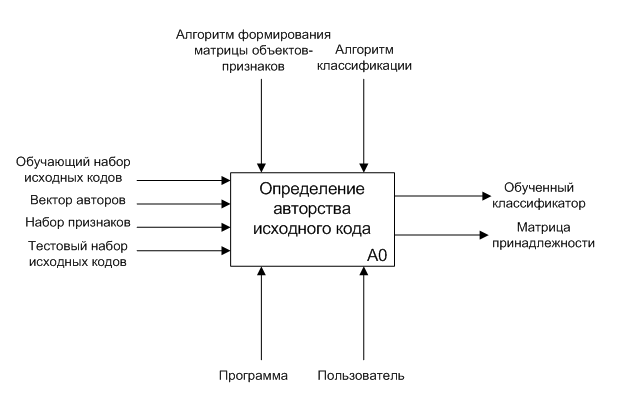
\includegraphics[width=0.9\linewidth]{box_1}}
\caption{ Модель <<черного ящика>> процесса определения авторства исходного кода по методологии IDEF0 }
\label{box_1:box_1}
\end{figure} 

\begin{figure}[h!]
\center{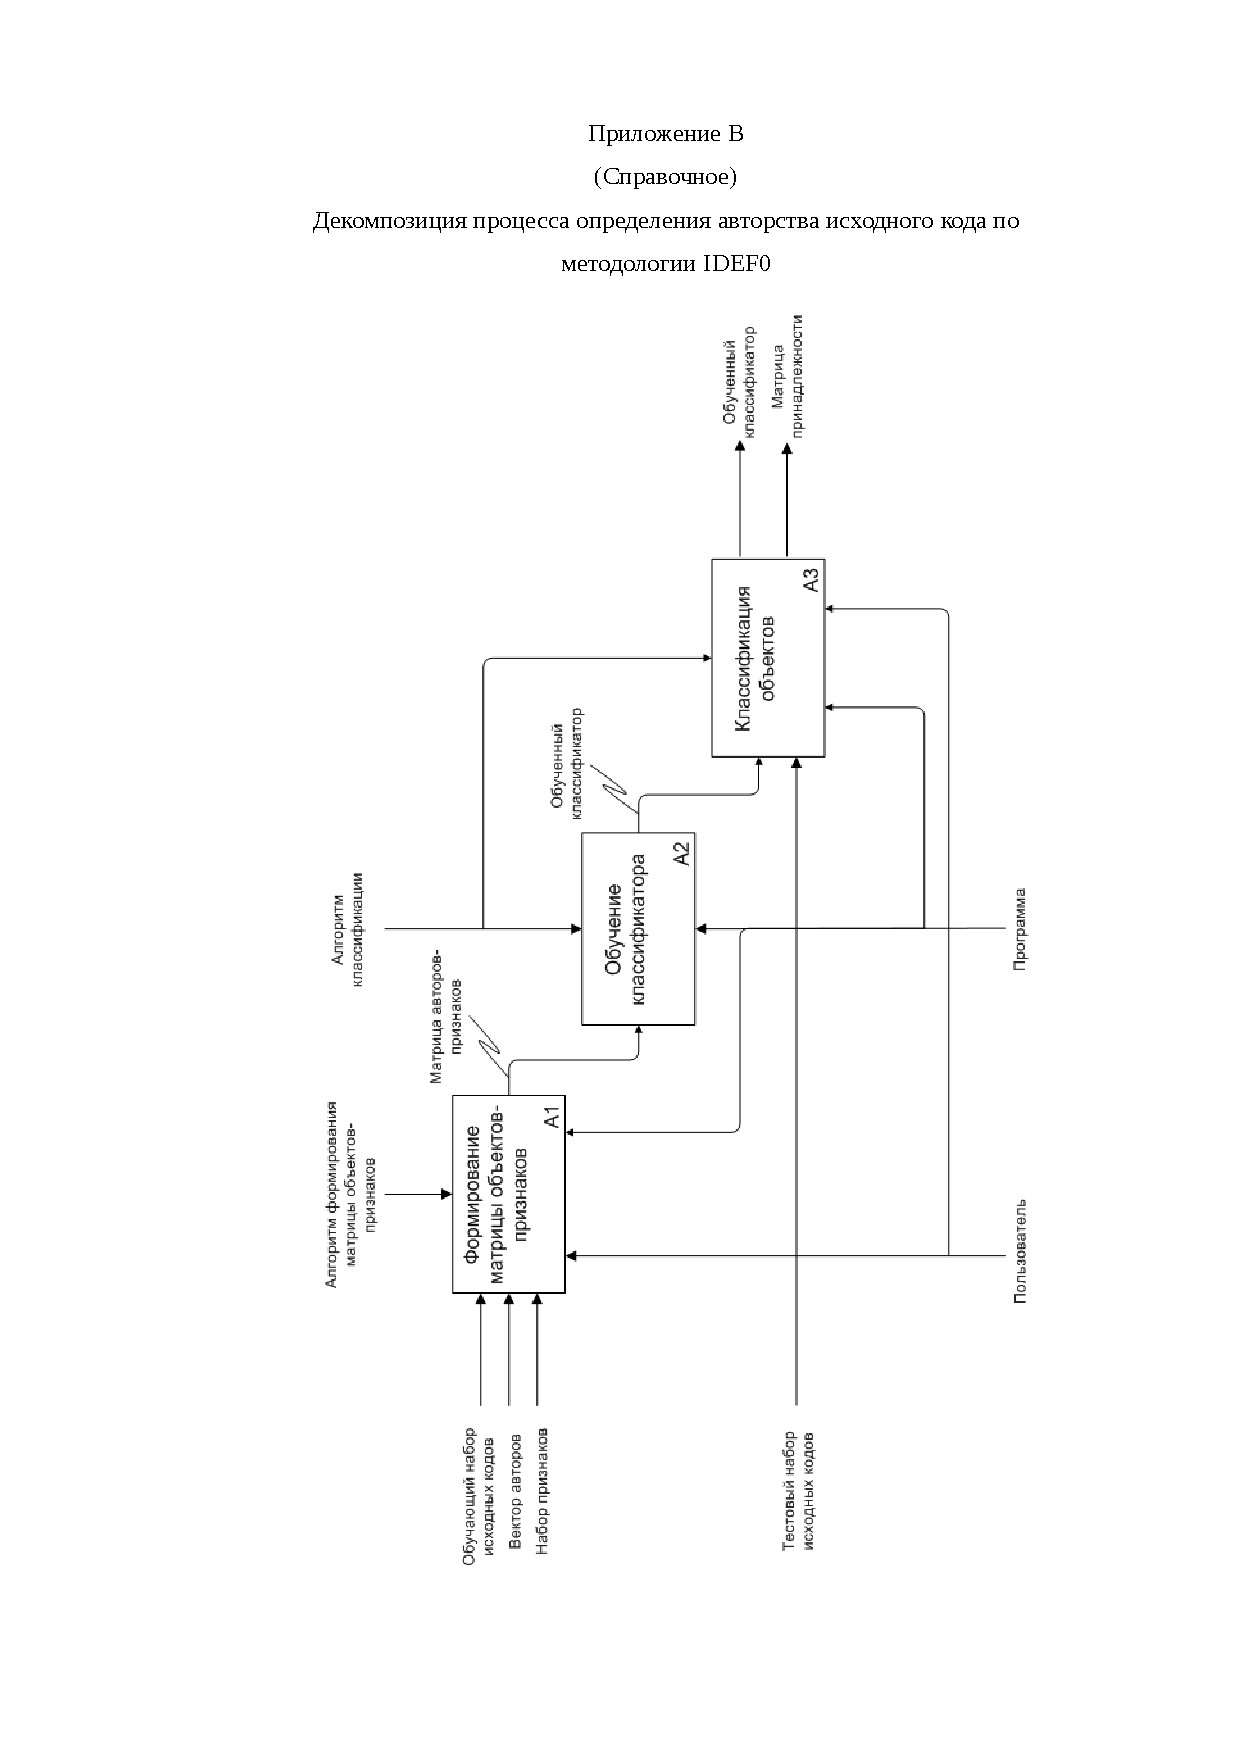
\includegraphics[width=1\linewidth]{box_2}}
\caption{ Декомпозиция <<черного ящика>> процесса определения авторства исходного кода по методологии IDEF0 }
\label{box_2:box_2}
\end{figure} 

\clearpage
 
 
\newpage  
\section{Классификация}\label{classifiers}
В данной работе в качестве базового алгоритма для всех классификаторов (см. разделы~\ref{random_forest},
\ref{ada}, \ref{extra}) были выбраны деревья решений 
(Decision Trees), тестирование и оценка модели производилась на основе 10-фолдовой кросс-валидации 
(см. раздел~\ref{crossval}).

Деревья решений (Decision Trees)~\cite{data_mining} или деревья принятия решений являются одним из наиболее популярных
методов решения задач классификации, регрессии и прогнозирования. Впервые деревья решений были предложены Ховилендом и Хантом (Hoveland, Hunt) 
в конце 50-х годов прошлого века и в наиболее простом виде представляют собой совокупность правил в иерархической 
структуре. Основа такой структуры --- это ветвление при проверке условий (<<Да>> --- <<Нет>>). 



\subsection{Алгоритм классификации Random Forest}\label{random_forest}
Алгоритм классификации Random Forest Classifier строится на двух базовых принципах: 
\begin{itemize}
  \item bagging --- мета-алгоритм в машинном обучении, при котором на основе большого числа <<слабых>> классификаторов (в данном случае деревьев решений) строится один <<сильный>> классификатор (рис.~\ref{forest:forest});
  \item метод случайных подпространств.
\end{itemize}

Преимущества данного алгоритма классификации:
\begin{itemize}
  \item способность эффективно обрабатывать данные с большим числом признаков и классов;
  \item нечувствительность к масштабированию (к любым монотонным преобразованиям) значений признаков;
  \item существует методы оценивания значимости отдельных признаков в модели;
  \item внутренняя оценка способности модели к обобщению (тест out-of-bag);
  \item высокая параллелизуемость и масштабируемость.
\end{itemize}

Недостатки алгоритма Random Forest Classifier:
\begin{itemize}
  \item алгоритм склонен к переобучению на некоторых задачах, особенно на зашумленных, однако для избежания переобучения используется энтропия Шеннона или коэффициент прироста информации (англ. Gain);
  \item большой размер получаемых моделей приводит к существенным затратам памяти на хранение деревьев, однако данный недостаток решается повышением вычислительных мощностей и распараллеливанием вычислений.~\cite{random_forest}
\end{itemize}

\begin{figure}[h!]
\center{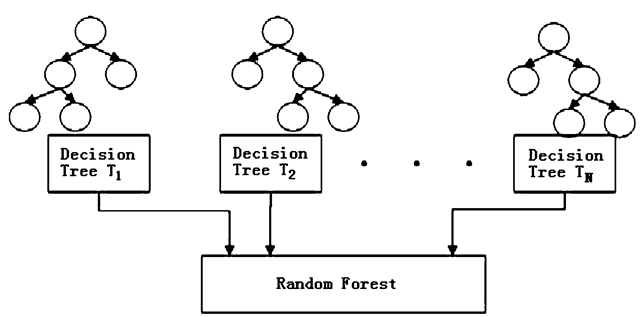
\includegraphics[width=0.7\linewidth]{forest}}
\caption{ Random Forest Classifier }
\label{forest:forest}
\end{figure} 

 

\subsection{Алгоритм классификации AdaBoost}\label{ada}
Алгоритм AdaBoost (сокр. от adaptive boosting)~\cite{ada_boost} является мета-алгоритмом, в процессе обучения 
строит композицию из базовых алгоритмов обучения для улучшения их эффективности.

Достоинства:
\begin{itemize}
 \item хорошая обобщающая способность --- в реальных задачах (не всегда, но часто) удаётся строить композиции, 
превосходящие по качеству базовые алгоритмы, при этом обобщающая способность может улучшаться (в некоторых задачах) 
по мере увеличения числа базовых алгоритмов;
 \item простота реализации;
 \item время построения композиции практически полностью определяется временем обучения базовых алгоритмов.
\end{itemize}


Недостатки алгоритма классификаций AdaBoost:
\begin{itemize}
 \item склонен к переобучению при наличии значительного уровня шума в данных;
 \item требует достаточно длинных обучающих выборок;
 \item бустинг может приводить к построению громоздких композиций, состоящих из сотен алгоритмов, 
 такие композиции исключают возможность содержательной интерпретации, требуют больших объёмов памяти 
 для хранения базовых алгоритмов и существенных затрат времени на вычисление классификаций.
\end{itemize}

\subsection{Алгоритм классификации ExtraTrees}\label{extra}
Алгоритм ExtraTrees (Extremly Randomized Trees) является модификацией 
алгоритма Random Forest Classifier (см. раздел~\ref{random_forest}), но отличается еще более рандомизированным
разделением входного набора данных на подвыборки. Как правило, результаты работы данного алгоритма
схожи с результатами Random Forest Classifier, однако в определенных случаях могут давать улучшение
точности классификации.~\cite{extra_trees}



\newpage
\section{Тестирование модели}\label{testing}
Раздел <<Программа и методика испытаний>> описывает тестирование

был составлен и оформлен в соответствии с ГОСТ 19.301--79.~\cite{gost_19301} 

\subsection{Объект испытаний}
\subsubsection{Полное наименование системы и ее условное обозначение}

Условное обозначение: <<WhoseCppCode>>.

\subsubsection{Область применения}

Разработанный программный комплекс можно использовать


\subsection{Цель испытаний}

Испытания системы предназначены для оценки адекватности модели, ее точности

\subsection{Требования к программе}

\subsection{Требования к программной документации}

Пояснительная записка к дипломной работе должна включать в себя:

\begin{itemize}
 \item задание по дипломному проектированию;
 \item руководство администратора (приложение~Г);
 \item руководство программиста (приложение~Д);
 \item руководство пользователя (приложение~Е):
 \item результаты вычислительных экспериментов.
\end{itemize}

руководство пользователя должно быть оформлено согласно~\cite{gost_19.505} 

программиста --- согласно~\cite{gost_19.504}  



\subsection{Средства и порядок испытаний}
\subsubsection{Технические и программные средства, используемые во время испытаний}



\subsubsection{Порядок проведения испытаний}


\subsection{Методы испытаний}\label{testing_methods}

В качестве методики тестирования применялась процедура кросс-валидации, описанная в разделе~\ref{crossval}.



\newpage 
\section{Описание тестового набора данных}\label{test_data}
Burrows в работе~\cite{burrows_big} выделяет следующие ключевые параметры тестовых данных,
которые могут влиять на точность классификации:

\begin{itemize}
 \item число авторов --- с увеличением числа авторов сложность классификации увеличивается, 
 точность --- снижается;
 \item число экземпляров выборки для каждого автора --- желательно соблюдать одинаковым для всех авторов во 
 избежание отклонения в сторону наиболее точно описанных авторов, а также иметь больше экземпляров 
 для увеличения размера тестовой выборки; 
 \item средняя длина образца кода (количество непустых строк кода) --- чем длиннее, тем выше точность
 классификации, изменение длины экземпляров выборки может влиять на отклонение в сторону наиболее 
 точно описанных авторов, однако не представляется возможным соблюдать длину экземпляра выборки постоянной;
 \item <<стилистическая зрелость>> (stylistic maturity) авторов --- уровень квалификации, 
 личные и профессиональные предпочтения в стиле написания программ;
 \item временные метки образцов кода --- подразумевается, что со временем программы устаревают, технологии
 и методы программирования меняются и, как следствие, изменяется стиль программирования;
 \item репрезентативность выборки --- демографические, социальные и другие факторы;
 \item типы авторов --- студент, фрилансер, профессиональный разработчик, 
 в идеале система должна включать в себя разные типы;
 \item языки программирования --- если тестировать несколько языков одновременно, 
 результат будет зависеть от характерных признаков языка;
 \item авторство в одном лице --- большинство проектов выполняются в 
 сотрудничестве с другими разработчиками;
 \item корректное авторство --- без плагиата, копирования и т.п.
\end{itemize}

Burrows упоминает также от том, что характерный стиль программирования нестабилен в начале карьеры программиста,
что может существенно отличать начинающего специалиста и профессионала разработки.

Программное обеспечение <<WhoseCppCode>> тестировалось на трех наборах данных:

\begin{enumerate}
 \item <<students>> --- выборка представляет собой работы студентов первого курса обучения по 
 предмету <<Основы программирования>>; все программы реализуют решения однотипных задач в рамках учебной 
 дисциплины, что исключет их разделение при классификации по функциональному назначению вместо 
 стилистических особенностей и снижение точности классификации; 
 \item <<Google Code Jam>> --- общедоступные данные ежегодной международной олимпиады по программированию Google Code Jam 
 2016~\cite{GoogleCodeJam}; так же, как и в первой выборке, авторы решали схожие задачи, используя различные
 подходы и алгоритмы; 
\item <<GitHub>> --- данные, собранные с сайта GitHub~\cite{GitHub}, крупнейшего~\cite{GH_domain} 
веб-сервиса для хостинга IT-проектов и их совместной разработки. 
\end{enumerate}


Сбор данных с веб-хостинга GitHub производился по следующему принципу: 
\begin{enumerate}
 \item выбирались крупные open-source репозитории,  
 посвященные разработке проектов на C/C++;
 \item просматривался список контрибьюторов;
 \item в качестве авторов выбирались те контрибьюторы, у которых имеются личные проекты, написанные 
 на C/C++;
 \item на основе списка пользователей автоматически, средствами программы <<WhoseCppCode>>, производился
 сбор и сохрание файлов исходного кода для каждого автора. 
\end{enumerate}

В таблице~\ref{tab:data} приводится описание некоторых характеристик каждого набора данных.
В данном случае под смешанным типом авторов подразумевается, что разработчики могли быть совершенно
разного уровня квалификации и рода деятельности (студенты, фрилансеры, начинающие и 
профессиональные разработчики, программисты-любители и т.д.).

\begin{table}[h!]
\caption{ Тестовые данные }
\label{tab:data}
\begin{center}
\begin{tabularx}{\linewidth}{|>{\hsize=0.4\hsize}X|>{\hsize=0.2\hsize}X|>{\hsize=0.2\hsize}X|>{\hsize=0.2\hsize}X|}
\hline
Набор данных & <<Students>> & <<Google Code Jam>> & <<GitHub>> \\
\hline
Число авторов & 3 & 30 & 30 \\
\hline
исло файлов исходного кода на одного автора & 14 & 9 & 78 \\
\hline
Всего файлов исходного кода & 42 & 278 & 2334 \\
\hline
Минимальное число строк кода & 33 & 36 & 26 \\
\hline
Максимальное число строк кода & 160 & 461 & 16348 \\
\hline
Среднее число строк кода на один файл исходного кода & 45 & 87 & 234 \\
\hline
Тип авторов & Студенты & Смешанный & Смешанный \\
\hline
\end{tabularx}
\end{center}
\end{table}


Каждая выборка представляет собой совокупность файлов исходного кода программ на языке C/C++ с расширениями
*.cpp, *.c, *.h, *.hpp, *.cxx, *.cc, *.ii, *.ixx, *.ipp, *.inl, *.txx, *.tpp, *.tpl.





\newpage
\section{Описание программного обеспечения <<WhoseCppCode>>}
Программное обеспечение <<WhoseCppCode>> состоит из двух основных частей:
\begin{itemize}
 \item программного модуля, реализующего все необходимые функции для сбора, анализа и обработки данных, 
а также построения модели классификации авторов исходного кода, описанной в разделе~\ref{modeling};
 \item программного интерфеса на основе технологии Jupyter Notebook~\cite{jupyter}, предназначенного 
 для визуализации полученных в ходе классификации результатов, сбора необходимых данных с ресурса GitHub~\cite{GitHub},
 построения матрицы объектов-признаков на основе входных данных, проведения вычислительных экспериментов.
\end{itemize}

Программный модуль реализован на языке прораммирования высокого уровня Python с использованием следующих 
программных библиотек:
\begin{itemize}
 \item Scikit-Learn~\cite{scikit} --- open-source библиотека для машинного обучения: классификации, регрессии, кластеризации и т.д.
 \item Plotly~\cite{plotly} --- графическая Python-библиотека для построения интерактивных графиков, таблиц, диаграмм.
 \item Numpy~\cite{numpy} --- библиотека для научных вычислений, предоставляющая методы работы с большими массивами данных.
 \item Scipy~\cite{scipy} --- предоставляет среду для проведения математических и научных вычислений.
 \item Pandas~\cite{pandas} --- open-source библиотека, предназначенная для анализа данных.
 \item Ipywidgets~\cite{widgets} --- интерактивные HTML виджеты для Jupyter Notebook.
\end{itemize}

Интерфейс основан на веб-технологиях, может использоваться для демонстрации возможностей
программ на языке Python. Библиотека Jupyter Notebook, с помощью которой был реализован
данный интерфейс, была выбрана за счет ряда преимуществ:
\begin{itemize}
 \item является свободным ПО;
 \item поддерживает множество языков программирования;
 \item позволяет хранить вместе код, изображения, комментарии, формулы и графики;
 \item не требует знаний и применения веб-технологий, таких как CSS, HTML, JavaScript;
 \item может быть запущен на любом сервере, необходим только доступ по ssh/http;
 \item позволяет экспортировать код и сам блокнот в любом формате;
 \item предназначена для демонстрации разработок на языке Python (в основном в машинном обучении).
\end{itemize}

Основной модуль программы <<WhoseCppCode>> может быть использован отдельно от Jupyter Notebook 
при разработке различного рода программ, систем и интерфейсов лицами, заинтересованными в задаче
классификации программистов.

Диаграмма действий в нотации UML, описывющая основной алгоритм работы программы <<WhoseCppCode>>
представлена на рисунке~\ref{flowchart:flowchart}, вид интерфейса программы --- 
на рисунках~\ref{user_notebook_1:user_notebook_1},~\ref{user_notebook_2:user_notebook_2},~\ref{user_notebook_3:user_notebook_3}
примеры ввода и вывода данных в интерфейсе Jupyter 
Notebook --- на рисунках~\ref{newplot:newplot} и~\ref{newplot2:newplot2}.
% 
\begin{figure}[ht!]
\center{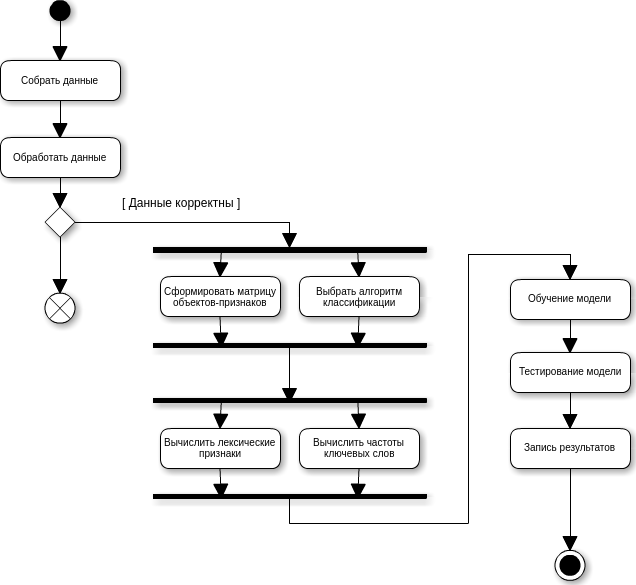
\includegraphics[width=0.8\linewidth]{flowchart}}
\caption{ Диаграмма действий алгоритма работы программы <<WhoseCppCode>> }
\label{flowchart:flowchart}
\end{figure}

\clearpage

\begin{figure}[ht!]
\center{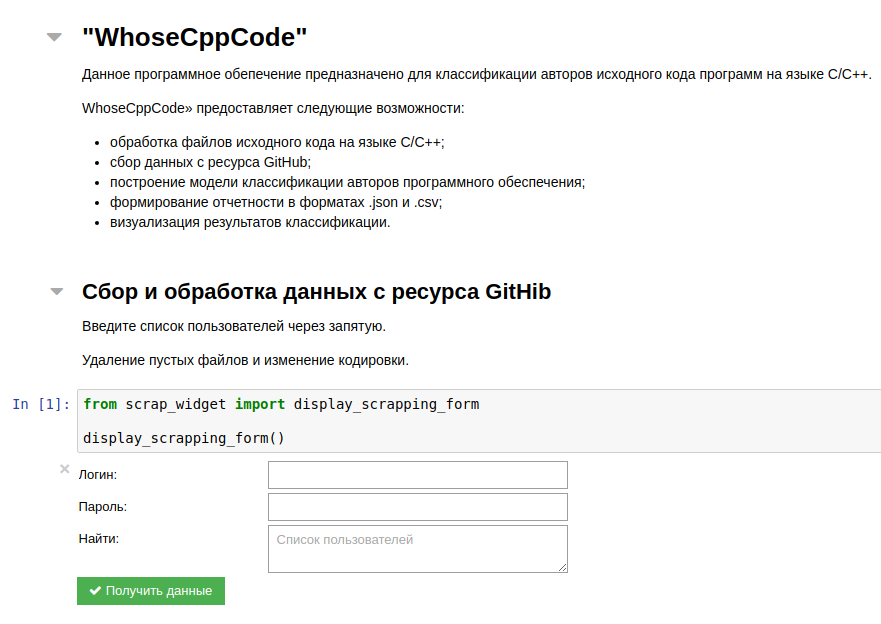
\includegraphics[width=0.9\linewidth]{user_notebook_1}}
\caption{ Вид программного интерфейса: сбор и обработка данных }
\label{user_notebook_1:user_notebook_1}
\end{figure}


\begin{figure}[ht!]
\center{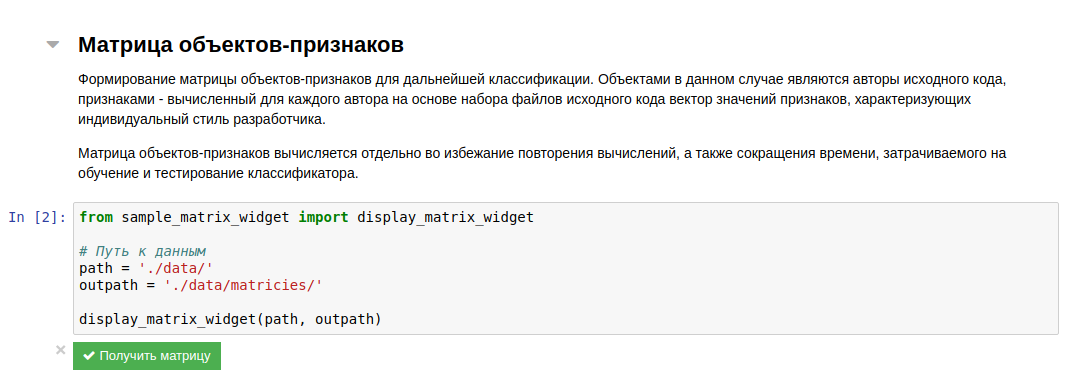
\includegraphics[width=1\linewidth]{user_notebook_2}}
\caption{ Вид программного интерфейса: формирование матрицы объектов-признаков }
\label{user_notebook_2:user_notebook_2}
\end{figure}

\clearpage

\begin{figure}[ht!]
\center{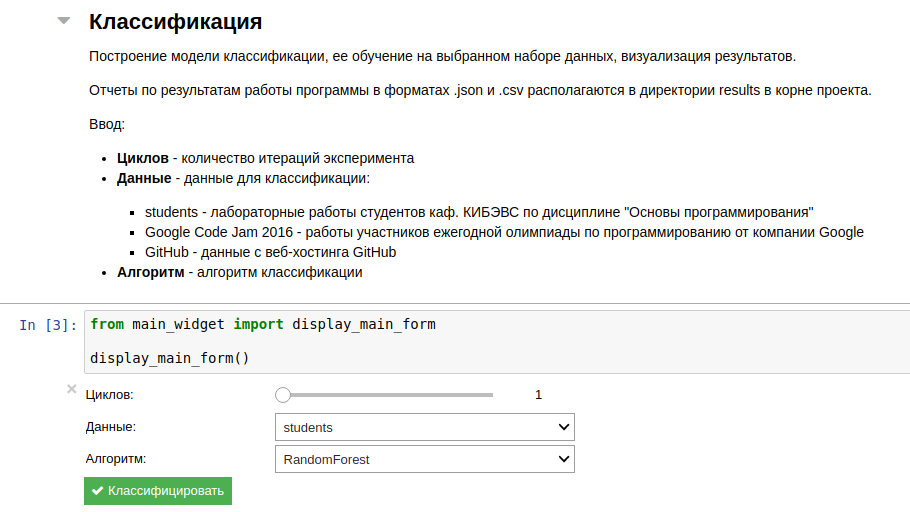
\includegraphics[width=1\linewidth]{user_notebook_3}}
\caption{ Вид программного интерфейса: классификация }
\label{user_notebook_3:user_notebook_3}
\end{figure}


\begin{figure}[h!]
\center{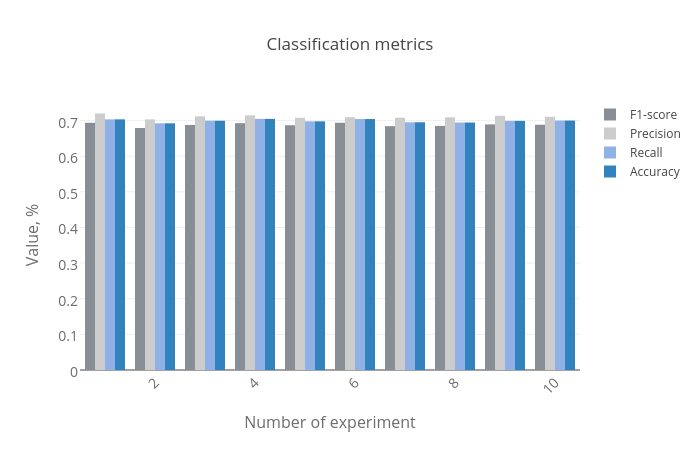
\includegraphics[width=0.7\linewidth]{newplot}}
\caption{ Вывод диаграммы результатов классификации }
\label{newplot:newplot}
\end{figure}


\begin{figure}[t!]
\center{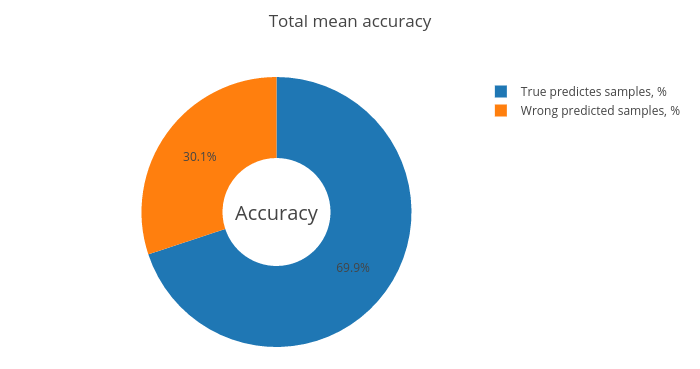
\includegraphics[width=0.7\linewidth]{newplot2}}
\caption{ Пример вывода диаграммы для средней точности классификации }
\label{newplot2:newplot2}
\end{figure}


\clearpage
% Описание функций, реализованных в основном модуле программы, а также
% примеры ввода и вывода данных в интерфейсе Jupyter Notebook представлены в приложениях Г и Д соответственно. 



\clearpage
\section{Критерии оценки эффективности классификации}\label{eval}
Критерии оценки работы классификатора~\cite{metrics} представлены в таблице~\ref{tab:eval}, где:
\begin{itemize}
  \item tp --- истинно-положительное решение;
  \item tn --- истинно-отрицательное решение;
  \item fp --- ложно-положительное решение;
  \item fn --- ложно-отрицательное решение;
  \item accuracy (точность) --- отношение количества документов, по которым классификатор принял правильное решение, к общему числу документов (примеров файлов исходного кода); 
  \item precision (правильность) --- доля документов, действительно принадлежащих данному классу, относительно всех документов, которые система отнесла к этому классу;
  \item recall (полнота) --- доля найденных классфикатором документов, принадлежащих классу, относительно всех документов этого класса в тестовой выборке;
  \item f1-score (f1-мера) --- гармоническое среднее между правильностью и полнотой.
\end{itemize}

\begin{table}[h!]
\caption{ Критерии оценки работы классификатора }
\label{tab:eval}
\begin{center}
\begin{tabularx}{\linewidth}{|c|c|X|X|}
\hline
Критерий & Формула & Луч. знач. & Худ. знач. \\
\hline
Accuracy (точность) & (tp + tn) / число примеров * 100 \% & 100 \% & 0 \% \\
\hline
Precision (правильность) & tp / (tp + fp) & 1 & 0 \\
\hline
Recall (полнота) & tp / (tp + fn) & 1 & 0 \\
\hline
F1-score (F1-мера) & 2 * (precision * recall) / (precision + recall) & 1 & 0 \\
\hline
\end{tabularx}
\end{center}
\end{table}

 
\newpage
\section{Результаты классификации}
При тестировании классификатора использовались критерии оценки, описанные в разделе~\ref{eval}, 
а также время работы программы. Результаты работы классификатора представлены в таблице~\ref{tab:results}, а также
на рисунках~\ref{students_res:students_res}, \ref{google:google} и~\ref{github:github}.

\begin{table}[h!]
\caption{ Результаты работы }
\label{tab:results}
\begin{center}
\begin{tabularx}{\linewidth}{|X|X|X|X|X|X|}
\hline
\multicolumn{6}{|c|}{Набор данных <<Students>>} \\
\hline
Классификатор & Accuracy, \% & Precision & Recall & F1-score & Время работы, сек.\\
\hline
RandomForest & 89,55 & 0,90 & 0,93 & 0,90 & 93,61\\
\hline
AdaBoost & 70,45 & 0,70 & 0,74 & 0,70 & 53,22\\
\hline
ExtraTrees & 91,85 & 0,92 & 0,95 & 0,92 & 53,70 \\
\hline
\multicolumn{6}{|c|}{Набор данных <<Google Code Jam>>} \\
\hline
Классификатор & Accuracy, \% & Precision & Recall & F1-score & Время работы, сек.\\
\hline
RandomForest & 86,66 & 0,86 & 0,88 & 0,87 & 110,65\\
\hline
AdaBoost & 19,43 & 0,16 & 0,16 & 0,19 & 103,53\\
\hline
ExtraTrees & 88,09 & 0,88 & 0,90 & 0,88 & 60,34 \\
\hline
\multicolumn{6}{|c|}{Набор данных <<GitHub>>} \\
\hline
Классификатор & Accuracy, \% & Precision & Recall & F1-score & Время работы, сек.\\
\hline
RandomForest & 69,92 & 0,69 & 0,71 & 0,70 & 223,77\\
\hline
AdaBoost & 16,44 & 0,09 & 0,11 & 0,16 & 451,63\\
\hline
ExtraTrees & 70,99 & 0,70 & 0,72 & 0,71 & 201,13 \\
\hline
\end{tabularx}
\end{center}
\end{table}

\begin{figure}[h!]
\center{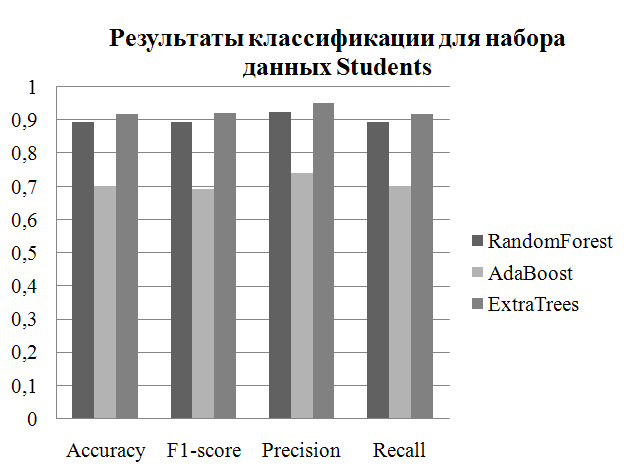
\includegraphics[width=0.6\linewidth]{students}}
\caption{ <<Students>> }
\label{students_res:students_res}
\end{figure}

\begin{figure}[h!]
\center{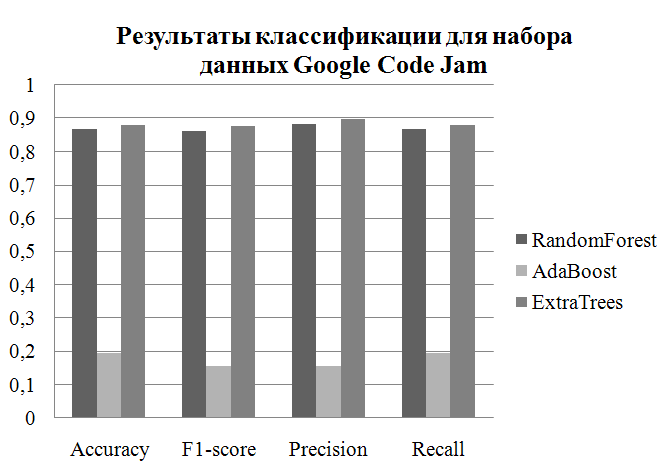
\includegraphics[width=0.6\linewidth]{google}}
\caption{ <<Google Code Jam>> }
\label{google:google}
\end{figure}

\begin{figure}[h!]
\center{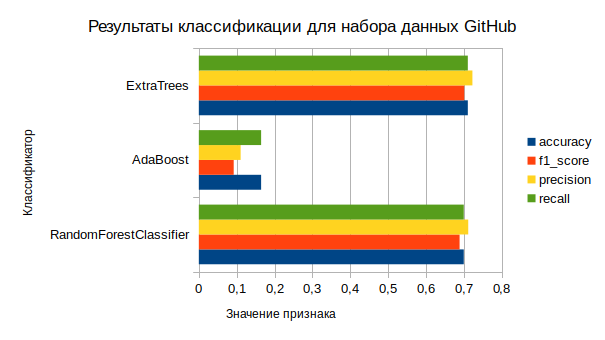
\includegraphics[width=0.6\linewidth]{github}}
\caption{ <<GitHub>> }
\label{github:github}
\end{figure}

Наихудшие результаты показал алгоритм AdaBoost, в то время как наиболее точным и быстрым из трех 
представленных алгоритмов оказался ExtraTrees (см. раздел~\ref{extra}). 

С использованием метода, основанного на извлечении лексических признаков и классификации с помощью алгоритма 
ExtraTrees (Extremly Randomized Trees) точность классификации составила 70-71 \% на выборке данных из 30 авторов
и 2334 неполных, немопилируемых файлов с веб-хостинга GitHub. 

По результатам классификации можно сделать
вывод, что данные методы могут применяться не только в <<лабораторных>> условиях, когда
тестовая выборка генерируется на основе студенческих работ или результатов олимпиад по программированию,
где решаются схожие задачи, ограниченные по времени и объему кода, но и в условиях реального мира.

\clearpage

% \newpage  
% \section{Руководство администратора}
% \input{admin}
% 
% \newpage  
% \section{Руководство программиста}
% \newpage
\setcounter{section}{0}
\section*{Приложение Д}
\section*{(Справочное)}
\section*{Руководство программиста}

\hfill

\begin{center}
 ПРОГРАММНОЕ ОБЕСПЕЧЕНИЕ ДЛЯ\\
 ОПРЕДЕЛЕНИЯ АВТОРСТВА ИСХОДНОГО КОДА ПРОГРАММ НА ЯЗЫКЕ С/С++\\
 <<WhoseCppCode>>\\
 
 Руководство программиста\\
 
 Листов 7
\end{center}


\hfill

\newpage
\section*{Аннотация}

\section{Назначение и условия применения программы}
\subsection{Назначение}

Программное обеспечение <<WhoseCppCode>> предназначено для определения авторства программ на 
языке С/С++ по исходному коду.

\subsection{Функции}

\subsection{Условия, необходимые для выполнения программы}

\section{Характеристики программного обеспечения}

\subsection{Режим работы}

\subsection{Описание особенностей программного обеспечения}

\subsection{Обеспечение надежности программного обеспечения}

\section{Обращение к программе}

\section{Алгоритм}


\section{Входные данные}

\section{Выходные данные}

\section{Сообщения}





% 
% \newpage  
% \section{Руководство пользователя}
% \begin{center}
 Приложение Е
 
 (Справочное)
 
 Руководство пользователя
\end{center}




\vspace*{7cm}
\begin{center}%
\LARGE {Lucas Kanade}\\\large{1.4}\\
\vspace*{1cm}
{\large Создано системой Doxygen 1.8.9.1}\\
\end{center}

\newpage
\section*{Введение}
\subsection{Область применения}
\subsection{}
\subsection{}
\subsection{}

\section{Назначение и условия применения}
\subsection{}
\subsection{}


\section{Подготовка к работе}
\subsection{}
\subsection{}
\subsection{}

\section{Описание операций}
\subsection{}
\subsection{}

\section{Аварийные ситуации}

\section{Рекомендации по освоению}






 
\newpage
\section*{Заключение}
\addcontentsline{toc}{section}{Заключение}
В ходе дипломного проектирования были выполнены все поставленные задачи:
\begin{itemize}
 \item проведен обзор актуальных информационных источников в области деанонимизации
 авторов программного обеспечения по его исходному коду;
 \item построена модель процесса определения авторства исходного кода;
 \item сформирован и обработан набор данных, состоящий из трех подвыборок, имеющих характерные особенности,
 которые оказывают влияние на точность классификации;
 \item произведена программная реализация разработанной модели и ее тестирование;
 \item разработан интерфейс на основе технологии Jupyter Notebook;
 \item проведены вычислительные эксперименты;
 \item произведен анализ полученных результатов;
 \item приведено технико-экономическое обоснование работы;
 \item рассмотрены вопросы безопасности жизнедеятельности.
\end{itemize}

Итогом дипломного проектирования является разработанное программное обеспечение <<WhoseCppCode>> на языке
программирования Python, предназначенное для сбора и обработки данных,
классификации авторов исходного кода на языке C/C++,
визуализации полученных результатов при помощи интерфейса. Основной программный модуль может быть использован
отдельно при разработке различных систем, интерфейсов и программ, а также дальнейших
научных исследований задачи деанонимизации авторов исходного кода. 



 
 
 \newpage
 \renewcommand{\refname}{Список использованных источников}
 \addcontentsline{toc}{section}{Список использованных источников}
 \bibliography{lit}

 \ESKDappendix{Обязательное}{\normalfont Компакт-диск}
 Компакт-диск содержит: 
 \begin{itemize}
 \item электронную версию пояснительной записки в форматах *.tex и *.pdf;
 \item итоговую презентацию результатов работы в форматах *.pptx и *.pdf;
 \item актуальную версию программы, реализованную на языке программирования Python, для определения авторсва исходного кода программ на языке C/C++;
 \item тестовые данные для работы с программой.
 \end{itemize}
 
 \ESKDappendix{Справочное}{\normalfont Сравнительный обзор информационных источников }
 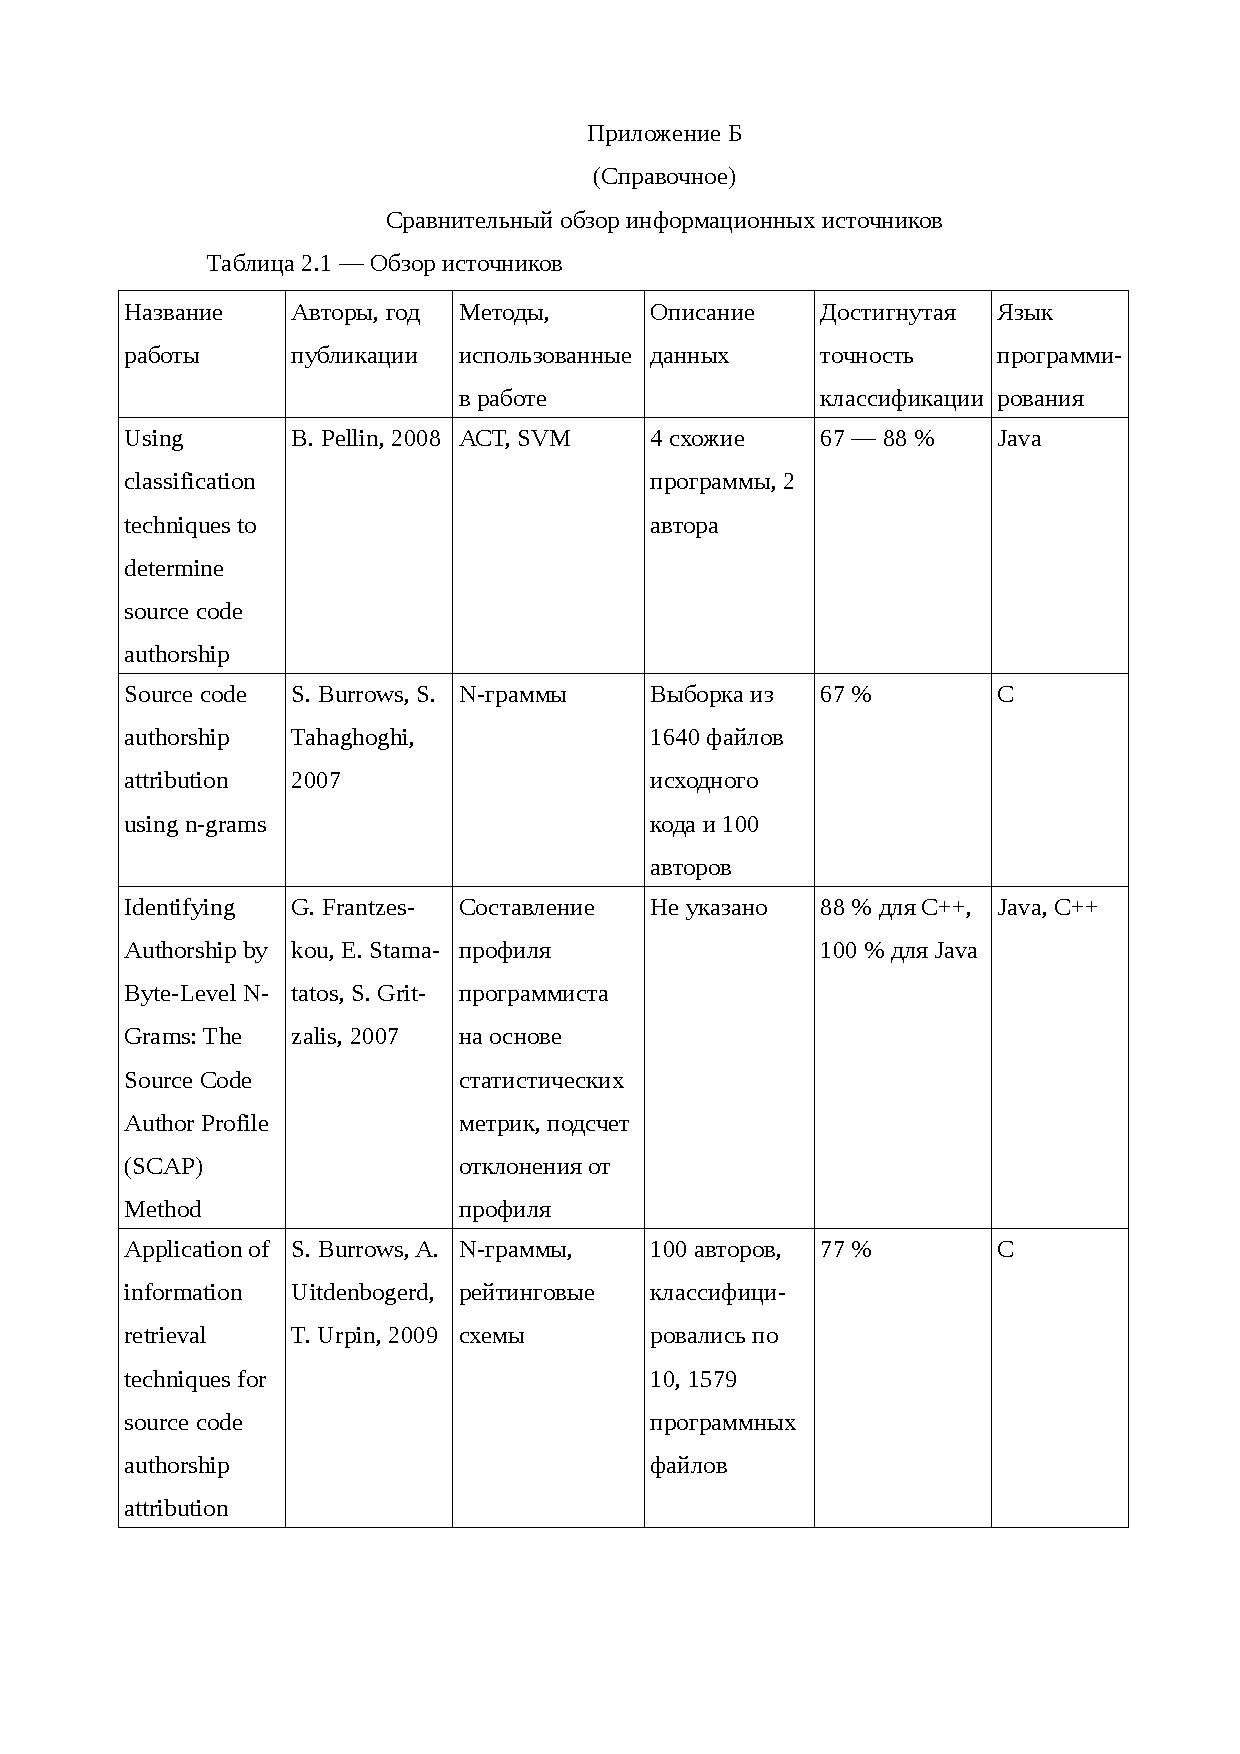
\includepdf[pages={1-2}]{overview_table}
 
 \ESKDappendix{Справочное}{\normalfont Описание стилистических признаков}
 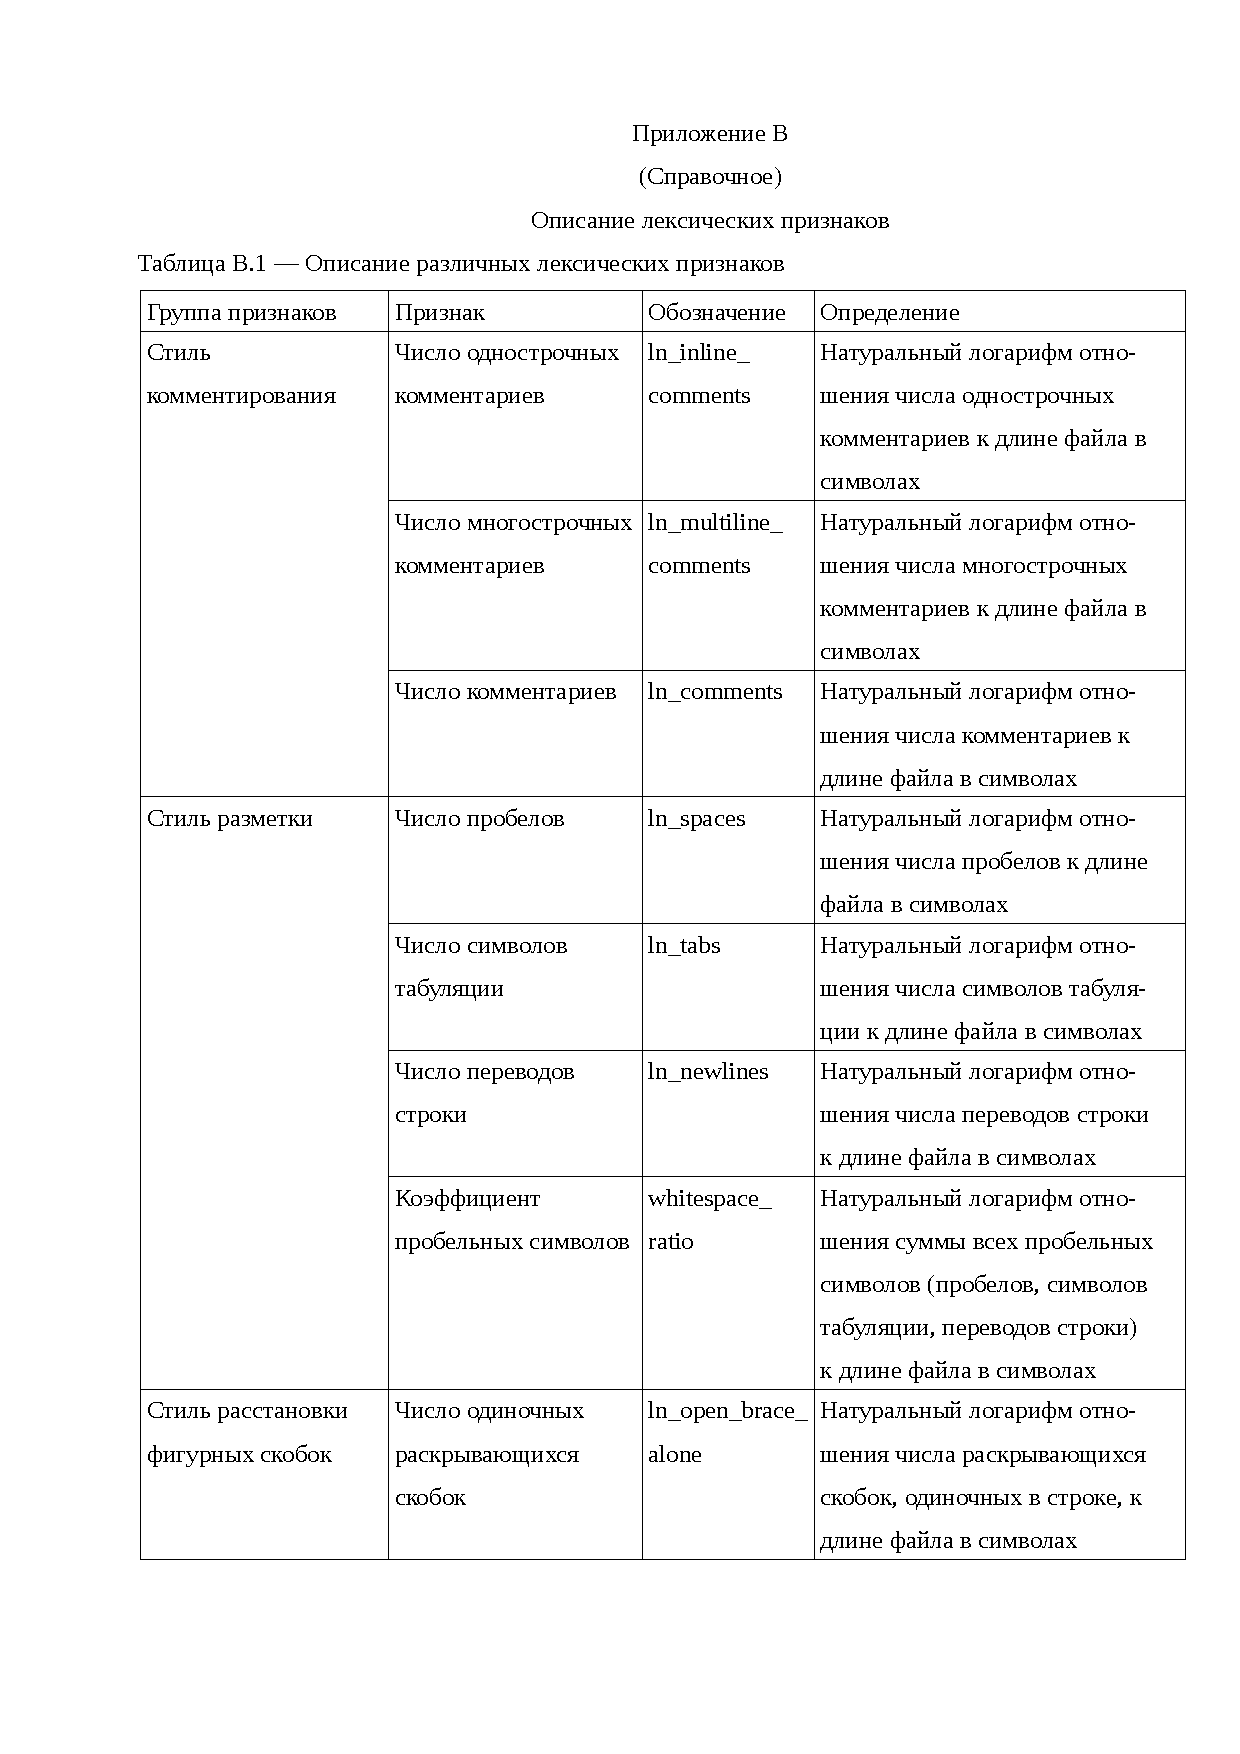
\includepdf[pages={1-2}]{lexical_features}
 
\end{document}
